\documentclass[]{book}
\usepackage{lmodern}
\usepackage{amssymb,amsmath}
\usepackage{ifxetex,ifluatex}
\usepackage{fixltx2e} % provides \textsubscript
\ifnum 0\ifxetex 1\fi\ifluatex 1\fi=0 % if pdftex
  \usepackage[T1]{fontenc}
  \usepackage[utf8]{inputenc}
\else % if luatex or xelatex
  \ifxetex
    \usepackage{mathspec}
  \else
    \usepackage{fontspec}
  \fi
  \defaultfontfeatures{Ligatures=TeX,Scale=MatchLowercase}
\fi
% use upquote if available, for straight quotes in verbatim environments
\IfFileExists{upquote.sty}{\usepackage{upquote}}{}
% use microtype if available
\IfFileExists{microtype.sty}{%
\usepackage{microtype}
\UseMicrotypeSet[protrusion]{basicmath} % disable protrusion for tt fonts
}{}
\usepackage[margin=1in]{geometry}
\usepackage{hyperref}
\hypersetup{unicode=true,
            pdftitle={Animal Environmental Science},
            pdfauthor={Sangrak Lee; Youngjun Na},
            pdfborder={0 0 0},
            breaklinks=true}
\urlstyle{same}  % don't use monospace font for urls
\usepackage{natbib}
\bibliographystyle{apalike}
\usepackage{longtable,booktabs}
\usepackage{graphicx,grffile}
\makeatletter
\def\maxwidth{\ifdim\Gin@nat@width>\linewidth\linewidth\else\Gin@nat@width\fi}
\def\maxheight{\ifdim\Gin@nat@height>\textheight\textheight\else\Gin@nat@height\fi}
\makeatother
% Scale images if necessary, so that they will not overflow the page
% margins by default, and it is still possible to overwrite the defaults
% using explicit options in \includegraphics[width, height, ...]{}
\setkeys{Gin}{width=\maxwidth,height=\maxheight,keepaspectratio}
\IfFileExists{parskip.sty}{%
\usepackage{parskip}
}{% else
\setlength{\parindent}{0pt}
\setlength{\parskip}{6pt plus 2pt minus 1pt}
}
\setlength{\emergencystretch}{3em}  % prevent overfull lines
\providecommand{\tightlist}{%
  \setlength{\itemsep}{0pt}\setlength{\parskip}{0pt}}
\setcounter{secnumdepth}{5}
% Redefines (sub)paragraphs to behave more like sections
\ifx\paragraph\undefined\else
\let\oldparagraph\paragraph
\renewcommand{\paragraph}[1]{\oldparagraph{#1}\mbox{}}
\fi
\ifx\subparagraph\undefined\else
\let\oldsubparagraph\subparagraph
\renewcommand{\subparagraph}[1]{\oldsubparagraph{#1}\mbox{}}
\fi

%%% Use protect on footnotes to avoid problems with footnotes in titles
\let\rmarkdownfootnote\footnote%
\def\footnote{\protect\rmarkdownfootnote}

%%% Change title format to be more compact
\usepackage{titling}

% Create subtitle command for use in maketitle
\newcommand{\subtitle}[1]{
  \posttitle{
    \begin{center}\large#1\end{center}
    }
}

\setlength{\droptitle}{-2em}

  \title{Animal Environmental Science}
    \pretitle{\vspace{\droptitle}\centering\huge}
  \posttitle{\par}
    \author{Sangrak Lee; Youngjun Na}
    \preauthor{\centering\large\emph}
  \postauthor{\par}
      \predate{\centering\large\emph}
  \postdate{\par}
    \date{Last update: 2019-02-14}

\usepackage{booktabs}

\begin{document}
\maketitle

{
\setcounter{tocdepth}{1}
\tableofcontents
}
\chapter*{Welcome}\label{welcome}
\addcontentsline{toc}{chapter}{Welcome}

This is the website for \textbf{``Animal environmental science''}. To
understanding individual animals, we have to understand the relationship
they have with their environment. This book will introduce the
interaction between animals and the environment.

This website is (and will always be) \textbf{free to use}, and is
licensed under the
\href{http://creativecommons.org/licenses/by-nc-nd/3.0/us/}{Creative
Commons Attribution-NonCommercial-NoDerivs 3.0} License. The book is
written in \href{https://rmarkdown.rstudio.com}{RMarkdown} with
\href{https://bookdown.org}{bookdown}. All photographs used in this book
was from \href{https://unsplash.com/}{Unsplash.com}. If you click the
download button up above, you can download the PDF version of the book.

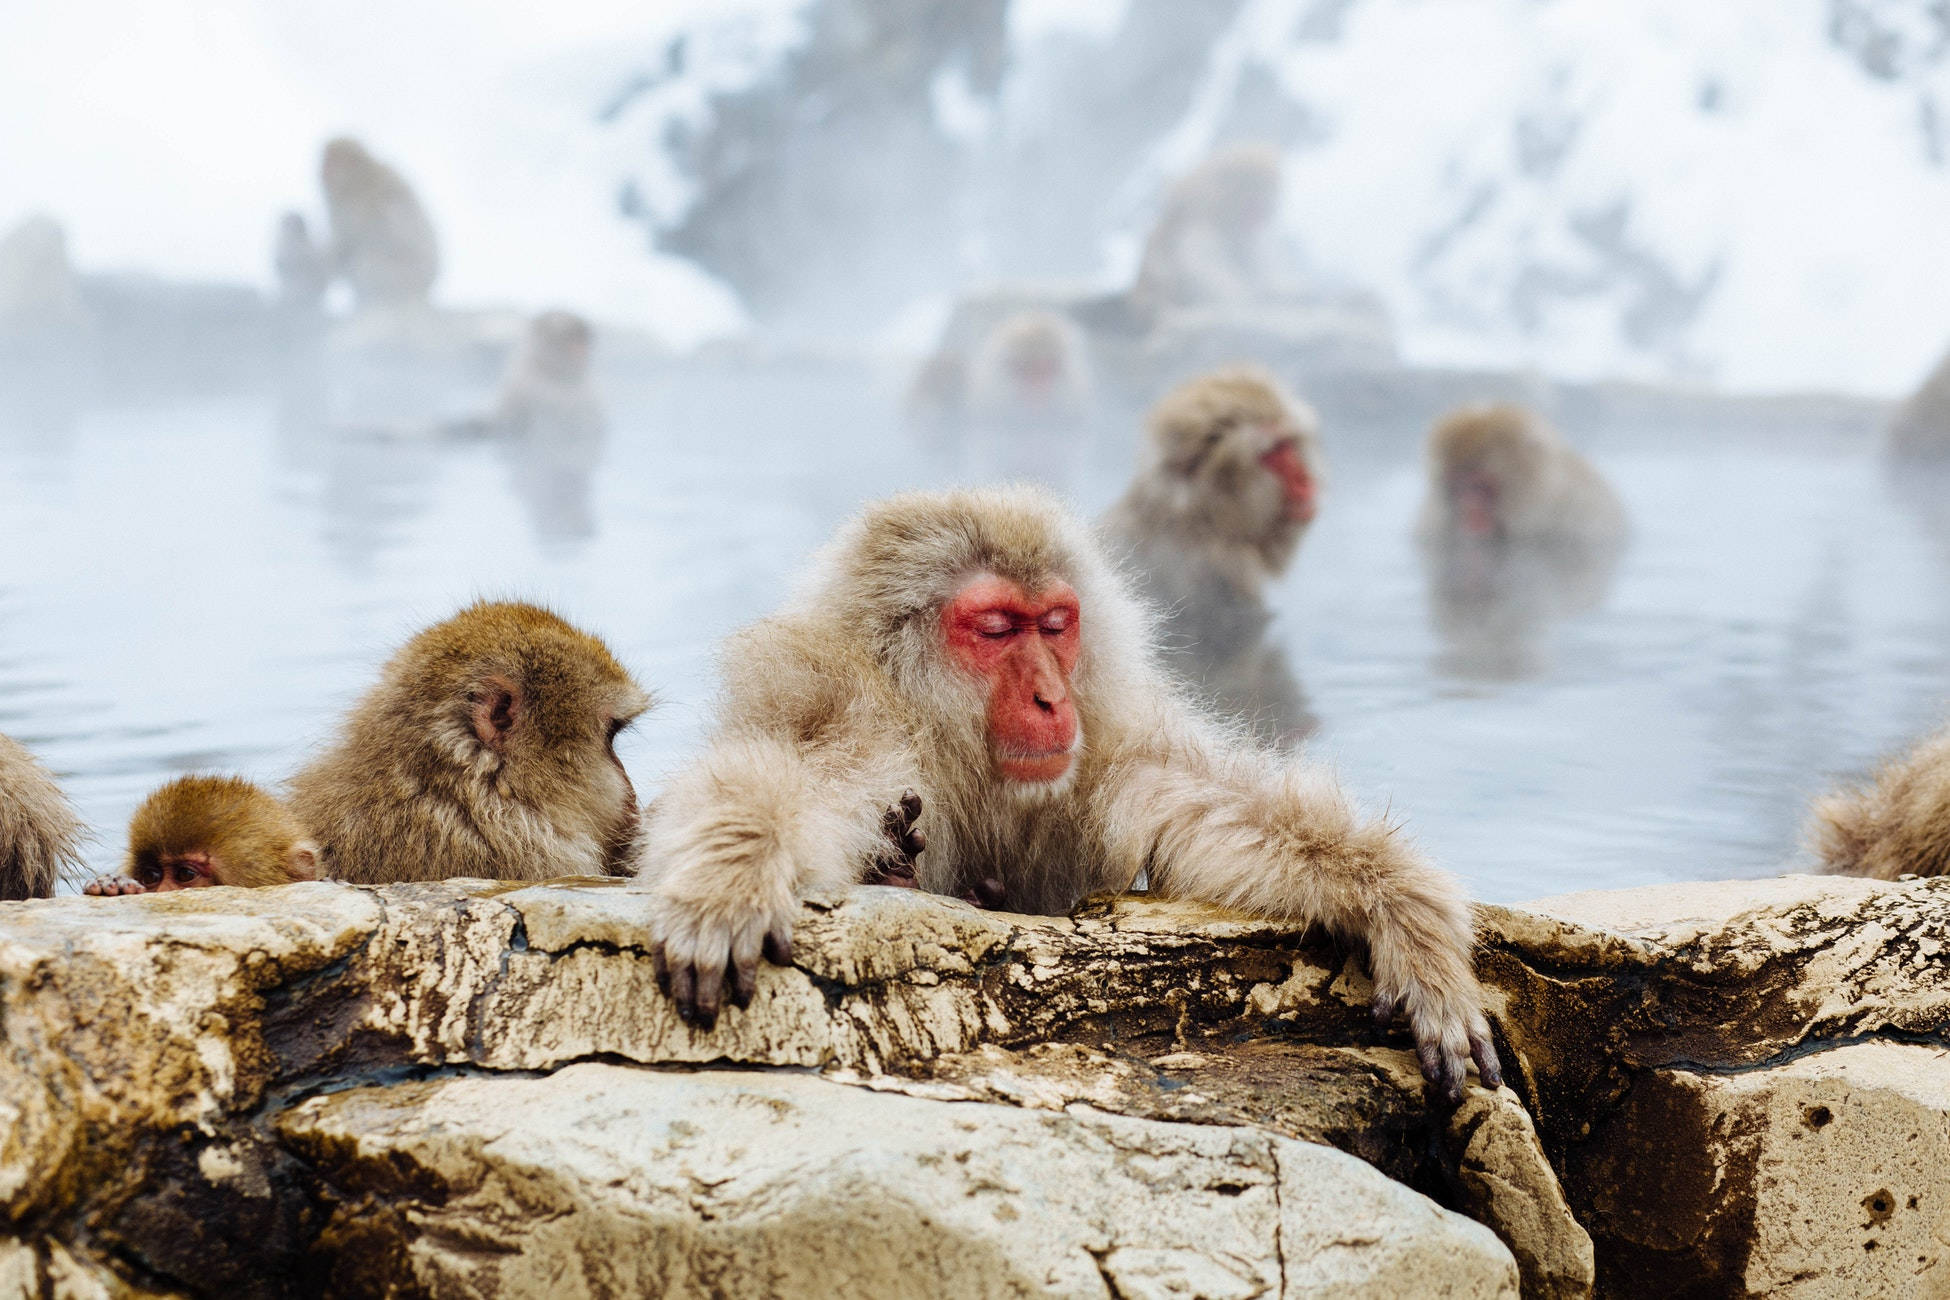
\includegraphics{figures/monkey.jpeg}\\
(Snow Monkey Niseko, Kutchan-chō, Japan)

\chapter{Introduction}\label{intro}

All living creatures constantly interact with the environment. To
understanding individual animals, we have to understand the relationship
they have with their environment. Basically, animals can find food,
shelter, protection, and mates from the environment called
\textbf{habitat}. The animal habitat includes both phisical (non-living)
and biotic (livinig) components (see Table \ref{tab:habitat}).

\begin{table}

\caption{\label{tab:habitat}Components of habitat (physical and biotic)}
\centering
\begin{tabular}[t]{ll}
\toprule
Physical & Biotic\\
\midrule
Temperature & Plant matter\\
Humidity & Predators\\
Oxygen & Parasites\\
Wind & Competitors\\
Soil & Individuals of the same species\\
\addlinespace
Light intensity & \\
Elevation & \\
\bottomrule
\end{tabular}
\end{table}

Animal habitat is constantly changed over time. Not only natural
disasters (eruption of volcano, earthquake, tsunami, and wildfire), also
human activity can affect the animal habitat. Unlike the wildlife, the
environment of domesticated animals (such as cow, pig, poultry, and dog)
that raised in facility are controlled by the human. Because it's a very
huge field, this book can't cover every topic of both wildlife and
domesticated animal. Thus, from now on, we will deal with the topic for
the domesticated animal.

\begin{figure}
\centering
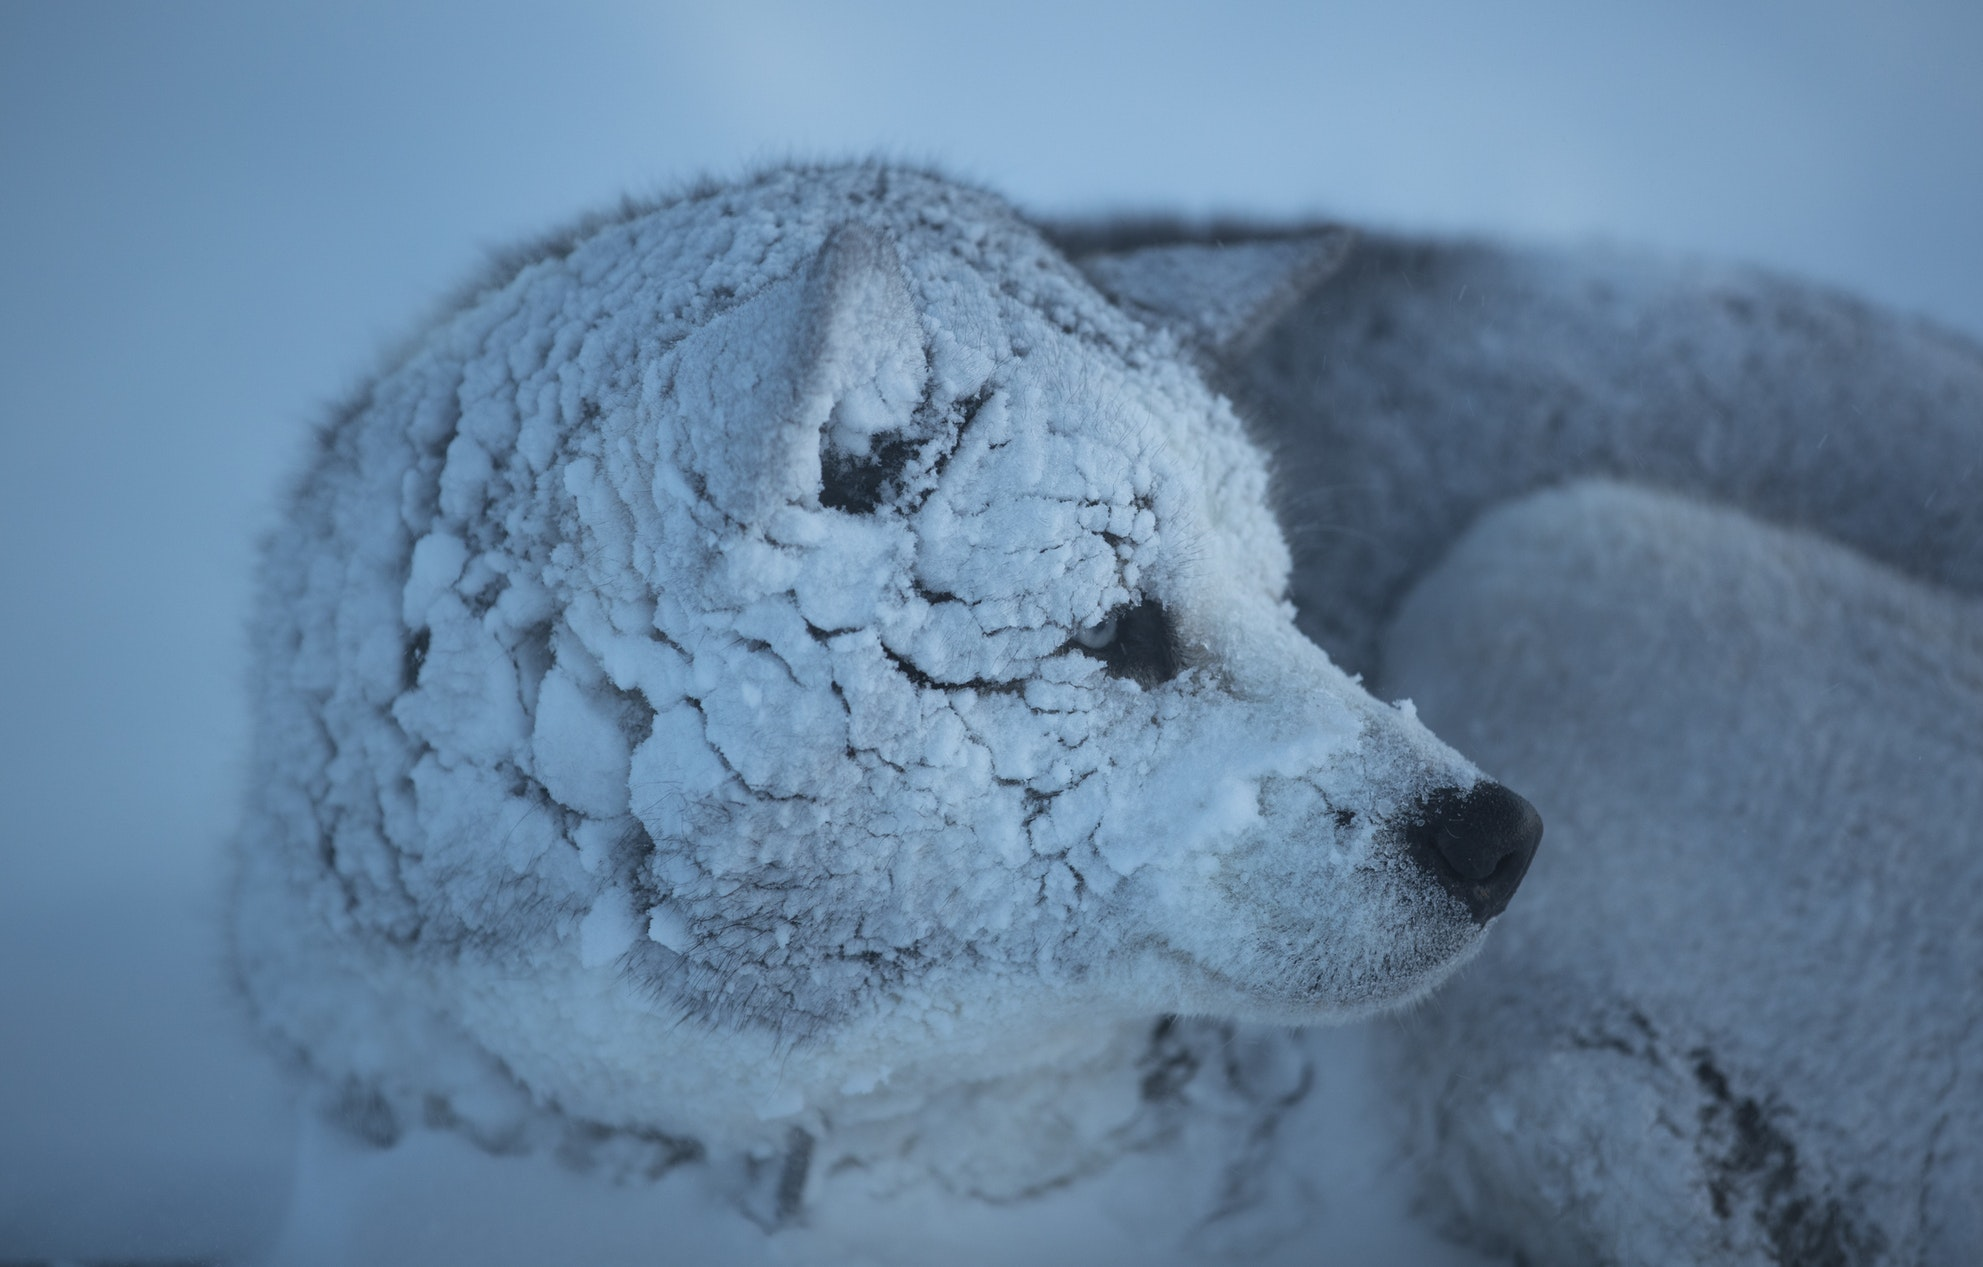
\includegraphics{figures/polar.jpeg}
\caption{}
\end{figure}

\chapter{Animal and environment}\label{chapter2}

\section{External environment}\label{external-environment}

Animal never separates from the stimuli from outside. In the domestic
animals, the external environment includes both physical (e.g.~housing,
feeder, paddock, fence, and noise) and biotic (e.g.~human, mate, and
feed ingredients) components like those of animal habitat \ref{intro}.

\begin{figure}
\centering
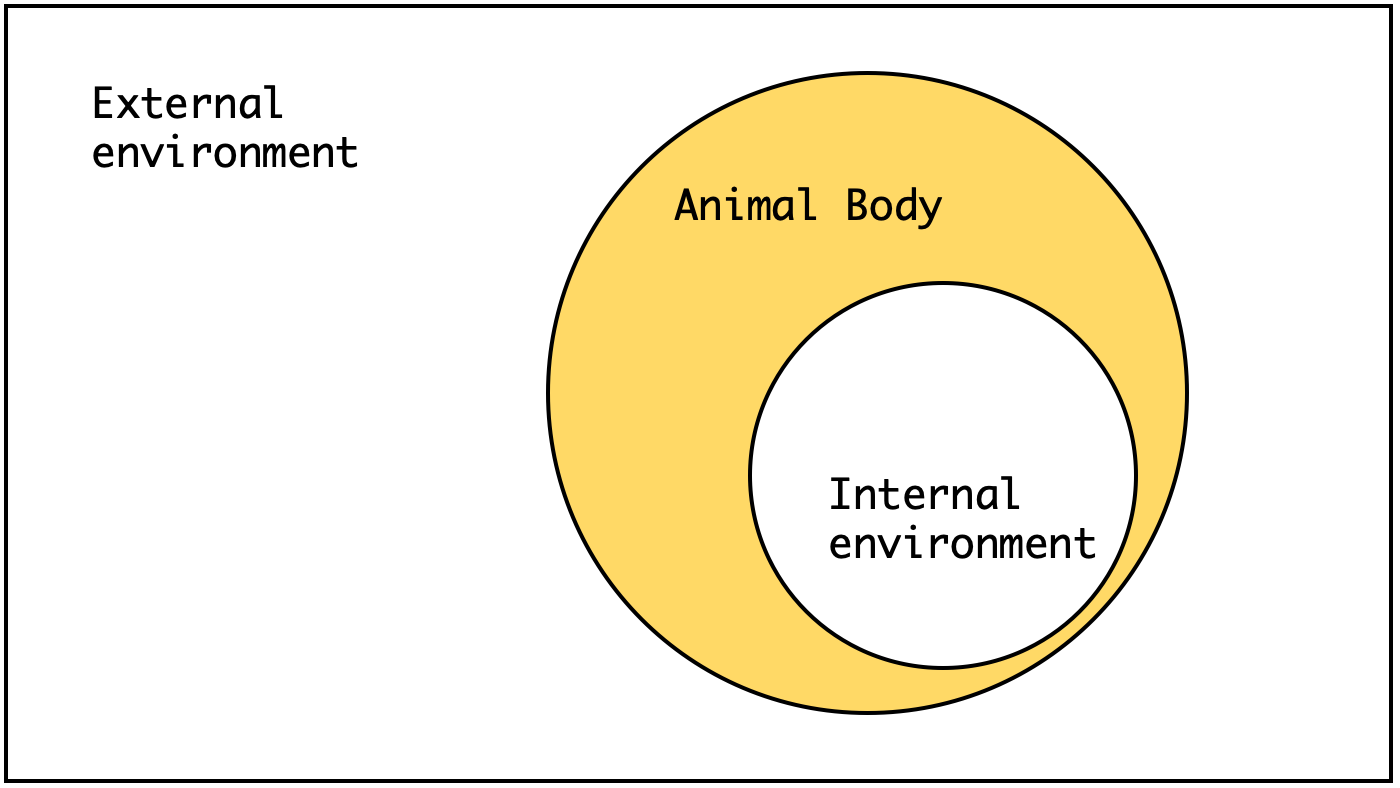
\includegraphics[width=0.60000\textwidth]{figures/animal-env.png}
\caption{}
\end{figure}

\section{Internal environment}\label{internal-environment}

\begin{quote}
``The living body, though it has need of the surrounding environment, is
nevertheless relatively independent of it.'' --- Claude Bernard
\end{quote}

Higher animals have complex organ systems that respond to stimuli to
perform their essential body functions. When the animal recieves the
signals from the sensory organs, they produce a local reflex action
and/or react in the central nervous system. Weak signals produce no
responses, but strong stimuli changes the physiological or behavioral
status of the animal.

\subsection{Shelford's law of
tolerance}\label{shelfords-law-of-tolerance}

\begin{quote}
``Each and every species is able to exist and reproduce successfully
only within a definite range of environmental conditions.'' --- Ronald
Good
\end{quote}

Although external environments are continuously changed, if animals in
the normal status, they keep the composition of the extracellular fluid
(internal environment) constant to maintain their live. We call it
\emph{homeostasis}. However, the capacity of to maintain the homeostasis
is broken when the animals let the harsh environments, and differ by
their species. \textbf{Animals may be limited in their growth and their
occurrence by the minimum, maximum, and optimum condition}
\citep{shelford} (Fig. \ref{fig:law-of-tol}).

\begin{table}

\caption{\label{tab:homeostasis}List of homeostatic control variables}
\centering
\begin{tabular}[t]{l}
\toprule
Control variables\\
\midrule
Core temperature; Blood glucose; Iron levels; Copper regulation; Levels of blood gases;\\
Blood oxygen content; Arterial blood pressure; Calcium levels; Sodium concentration;\\
Potassium concentration; Fluid balance; Blood pH; Cerebrospinal fluid; Neurotransmission;\\
Neuroendocrine system; Gene regulation; and Energy balance\\
\bottomrule
\end{tabular}
\end{table}

\begin{figure}
\centering
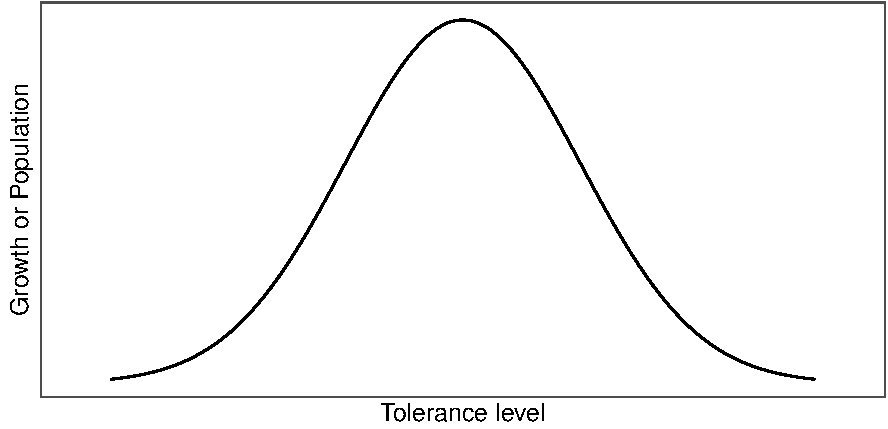
\includegraphics{AES_files/figure-latex/law-of-tol-1.pdf}
\caption{\label{fig:law-of-tol}Shelford's law of tolerance}
\end{figure}

The optimum range of environmental condition may differ within the same
organism, and it is not necessarily fixed. They can change as:

\begin{itemize}
\tightlist
\item
  Change of seasons
\item
  Change of environmental conditions
\item
  Life stage of the organism
\end{itemize}

\subsection{Adaptation}\label{adaptation}

\begin{quote}
``Changes in morphological, anatomical, physiological, biochemical and
behavioral characteristics of the animal which promote welfare and favor
survival in a specific environment.'' --- Hafez
\end{quote}

\citet{hafez1968adaptation} defined an adaptation as above. The
adaptation helps an animal survive in their external environment. The
representative adaptive traits are:

\begin{enumerate}
\def\labelenumi{\arabic{enumi}.}
\tightlist
\item
  Structural adaptation
\item
  Behavioural adaptation
\item
  Physiological adaptation
\end{enumerate}

Structural adaptation is the changes in physical features (e.g.~body
shape, skin, and internal organs) of the animal. Behavioural adaptation
is the changes in behaviours (e.g.~searching for food, mating,
vocalizations, and mitigation) of the animal. Physiological adaptation
is the changes in the animal body functions such as growth, temperature
regulation, and ionic balance. Sometimes, adapted animal create a new
species (\emph{speciation}).

\subsection{Acclimatization}\label{acclimatization}

Acclimatization is the physiological changes induced by a complex of
factors such as altitude, temperature, humidity, photoperiod, or pH.
Acclimatization is the short-term process (hours to weeks) by comparison
with adaptation (take place over many generations).

\part{Environmental effects on
animals}\label{part-environmental-effects-on-animals}

\chapter{Temperature}\label{temperature}

All chemical reactions are affected by temperature. Especially,

\section{Poikilotherm and
homoiotherm}\label{poikilotherm-and-homoiotherm}

\section{Thermoregulation}\label{thermoregulation}

\section{Temperature humadity index
(THI)}\label{temperature-humadity-index-thi}

\section{Effects on production}\label{effects-on-production}

\subsection{Dairy cattle}\label{dairy-cattle}

\subsection{Beef cattle}\label{beef-cattle}

\subsection{Swine}\label{swine}

\subsection{Poultry}\label{poultry}

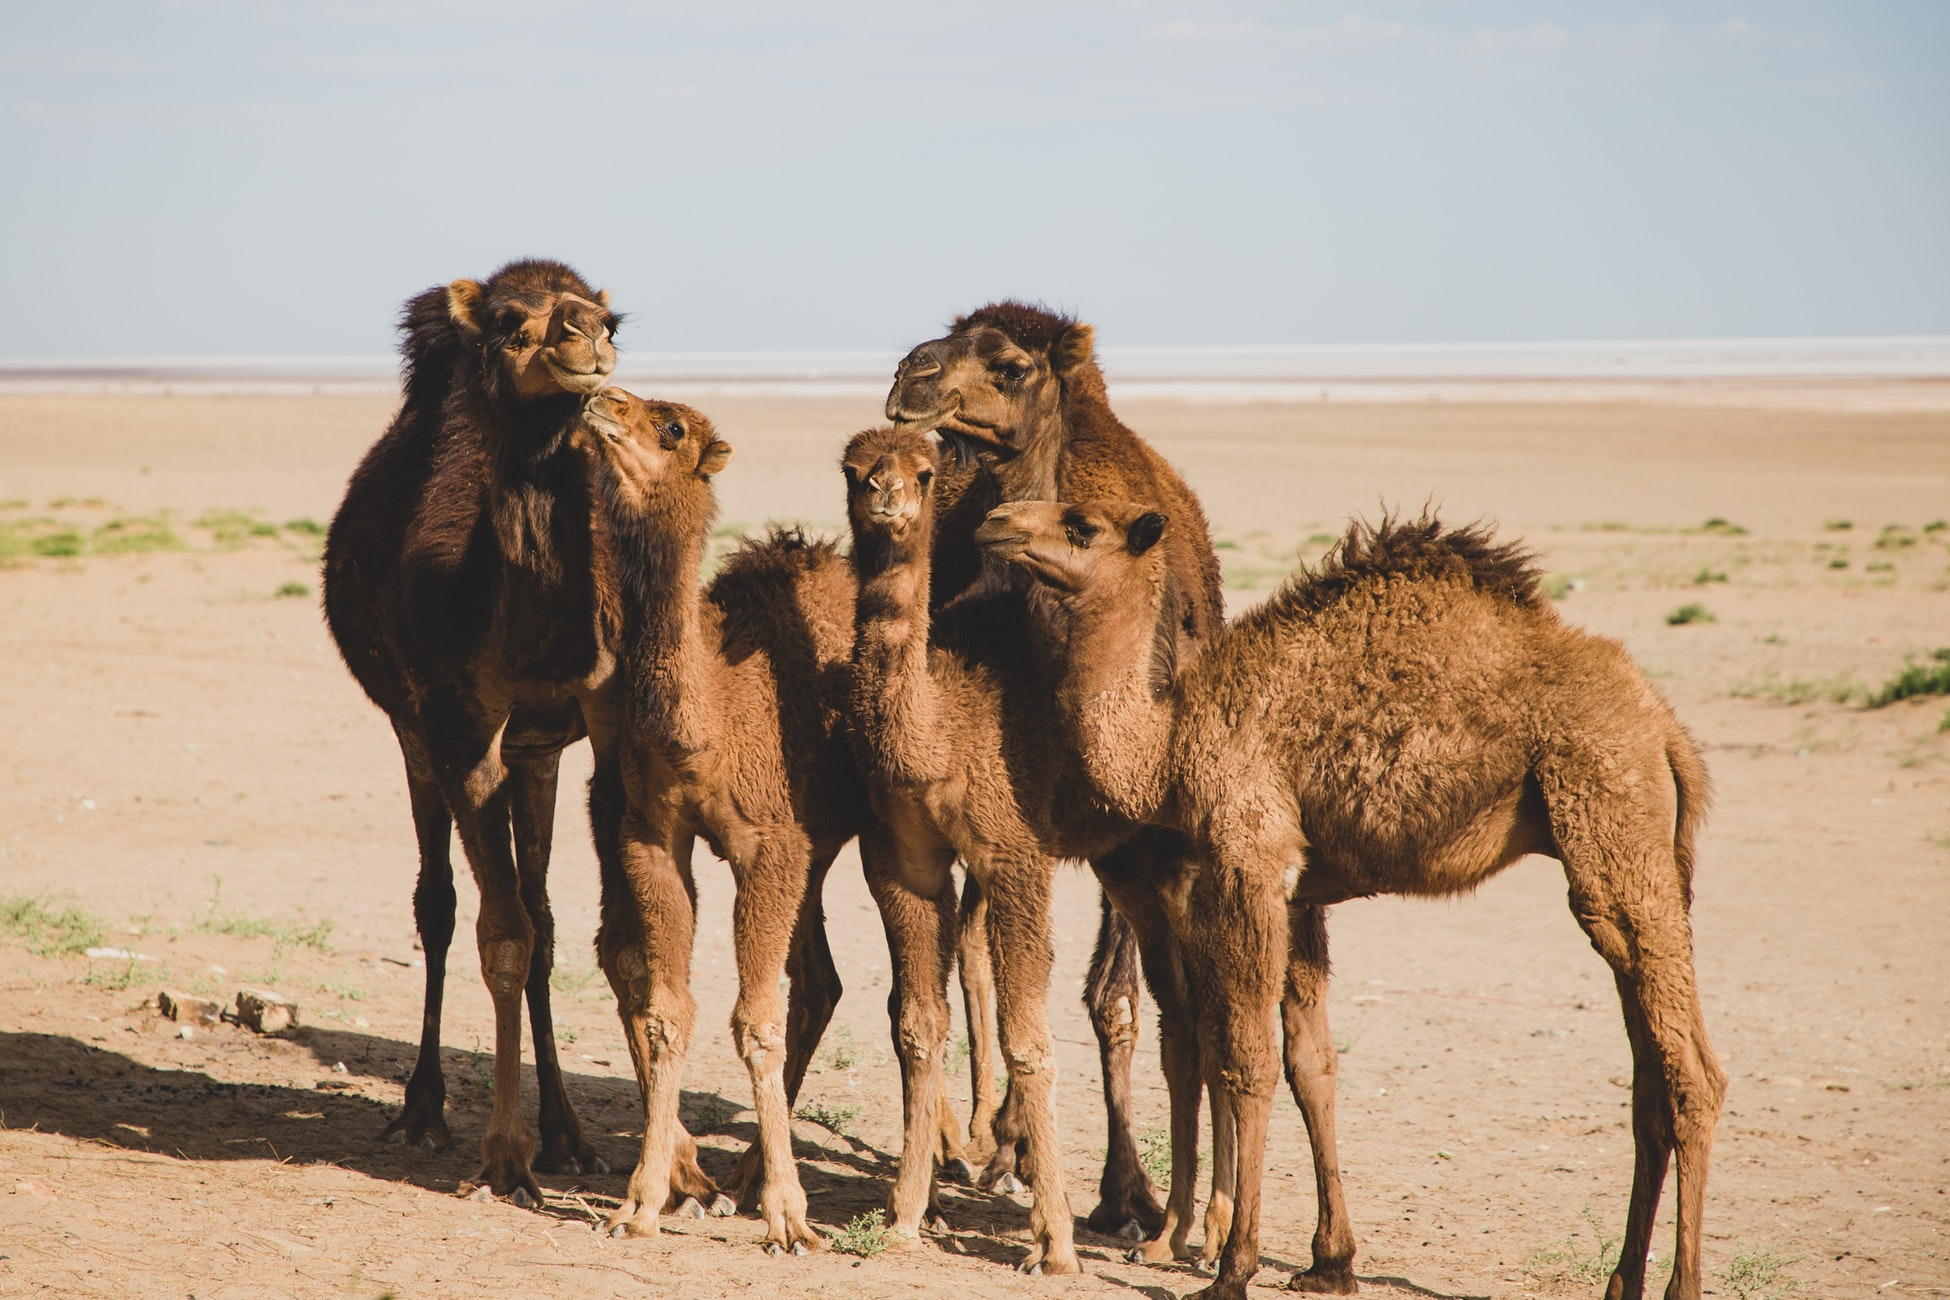
\includegraphics{figures/camels.jpeg} (Isfahan Province, Aran o Bidgol,
Iran)

\chapter{Light}\label{light}

\section{Photoperiodic response}\label{photoperiodic-response}

\section{Effects on productivity}\label{effects-on-productivity}

\subsection{Wool}\label{wool}

\subsection{Feathers}\label{feathers}

\subsection{Antlers}\label{antlers}

\subsection{Puberty}\label{puberty}

\subsection{Reproduction}\label{reproduction}

\subsection{Behavior}\label{behavior}

\subsection{Light control in poultry
production}\label{light-control-in-poultry-production}

\chapter{Sound}\label{sound}

\chapter{Air quality}\label{air-quality}

\chapter{Water quality}\label{water-quality}

\part{Animal effects on the
environment}\label{part-animal-effects-on-the-environment}

\chapter{Cycles of materials}\label{cycles-of-materials}

\section{Ecosystem}\label{ecosystem}

\section{Trophic level}\label{trophic-level}

\section{Carbon cycle}\label{carbon-cycle}

\section{Nitrogen cycle}\label{nitrogen-cycle}

\section{P and Ca cycle}\label{p-and-ca-cycle}

\chapter{Manure}\label{manure}

\section{Charateristics of animal
manure}\label{charateristics-of-animal-manure}

\section{Manure treatment}\label{manure-treatment}

\subsection{Composting}\label{composting}

\subsection{Liquid fertilizer}\label{liquid-fertilizer}

\subsection{Purification}\label{purification}

\subsection{Energy generation}\label{energy-generation}

\subsection{Animal feed}\label{animal-feed}

\chapter{Greenhouse gases}\label{greenhouse-gases}

Here is a review of existing methods.

\part{Sustainable livestock
industry}\label{part-sustainable-livestock-industry}

\chapter{Animal welfare}\label{animal-welfare}

Here is a review of existing methods.

\chapter{Sustainable livestock
industry}\label{sustainable-livestock-industry}

\begin{quote}
``In essence, the conflict between livestock and the environment is a
conflict between different human needs and expectations.'' --- Henning
Steinfeld (FAO)
\end{quote}

\bibliography{book.bib,packages.bib}


\end{document}
